\section{Wireframe}\label{s:wireframe}
La realizzazione dei wireframe è stata fatta mediante il software \textit{Balsamiq}; la loro realizzazione ha attraversato diverse iterazioni. Nelle seguenti sezioni presenteremo i vari wireframe e i widget che li compongono spiegando quali sono stati i nostri ragionamenti e le nostre iterazioni per raggiungere la versione finale.\\

\subsubsection{Header e footer}\label{ss:header-e-footer}
Ogni schermata possiede un header nella parte alta dello schermo e un footer nella parte bassa. I footer sono tutti uguali uguali, gli header sono simili in quanto presentano tutti un selettore di data, l'unico che differisce è quello della schermata ``Analisi di periodi'' che ne presenta due in quanto in quella schermata deve essere possibile, per il giornalista, inseire due range di date.

\begin{figure}[H]
    \centering
    
\includegraphics[width=1\columnwidth]{wireframes/header-una-data}
    \caption{Header di ``Panoramica'', ``Confronto fra regioni'' e ``Distribuzione su dati anagrafici''.}
    \label{fig:header-una-data}
\end{figure}

\begin{figure}[H]
    \centering
    
\includegraphics[width=1\columnwidth]{wireframes/header-due-date}
    \caption{Header di ``Analisi di periodi''.}
    \label{fig:header-due-date}
\end{figure}

Gli headers sono composti, partendo da destra:
\begin{itemize}
    \item logo della protezione civile;
    \item titolo della dashboard;
    \item pulsante per aprire il menù per selezionare quali widget visualizzare;
    \item pulsante per salvare in locale la vista e l'organizzazione della schermata aperta in quel momento;
    \item pulsante per caricare, e aprire, una schermata, e la sua organizzazione, salvata in precedenza o condivisa da un altro utilizzatore della dashboard;
    \item selettore di date (due in \ref{fig:header-due-date}) composto da:
        \begin{itemize}
            \item freccia a sinistra, un bottone per passare al giorno precedente a quello indicato;
            \item bottone per aprire il widget per selezionare la data (\ref{} e \ref{});
            \item freccia a destra, simile alla freccia a sinistra ma con comportamento opposoto, cambia la data al giorno successivo rispetto a quello indicato (se la da ta è valida).
        \end{itemize}
\end{itemize}

\paragraph{Seleziona metriche}
Il pulsante ``Seleziona metriche'' è stato aggiunto per permettere all'utilizzatore della dashboard di selezionare quali metriche vuole avere all'interna dall schermata. Al suo click compare una lista (\ref{fig:seleziona-metriche}) con tutte le metriche disponibili per quella schermata; l'utente può trascinare una metrica dalla lista all'interno della schermata e rilasciarla in una posizione compatibile andando così a sostituire una delle metriche presenti. Le posizioni compatibili con la metrica trascinata vengono evidenziate in quanto le uniche a colori e con una griglia attorno. Una metrica già presente all'interno della schermata, indicata da una spunta (\checkmark) non sono trascinabili all'interno della schermata, e, in caso di tentativo viene mostrato un avviso all'utente. In caso l'utente clicchi semplicemente su una metrica invece di trascinarla, compare un tooltip sulla metrica cliccata che spiega il funzionamento della meccanica (\ref{fig:seleziona-metriche-tooltip}). \`E in oltre presente un pulsante per ripristinare la schermata alle metriche di default, questo pulsante ha l'etichetta ``Ripristina le metriche di default''.

\begin{figure}[H]
    \begin{subfigure}[b]{0.5\textwidth}
        \centering
        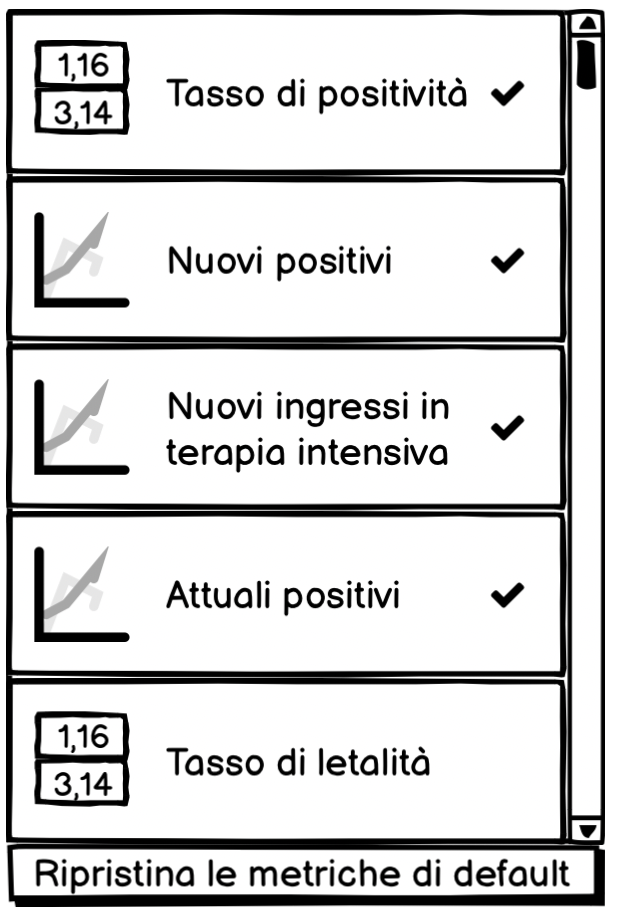
\includegraphics[width=0.3\textwidth]{wireframes/seleziona-metriche}
        \caption{Menù di selezione delle metriche.}
        \label{fig:seleziona-metriche}
    \end{subfigure}
\hfill
    \begin{subfigure}[b]{0.5\textwidth}
        \centering
        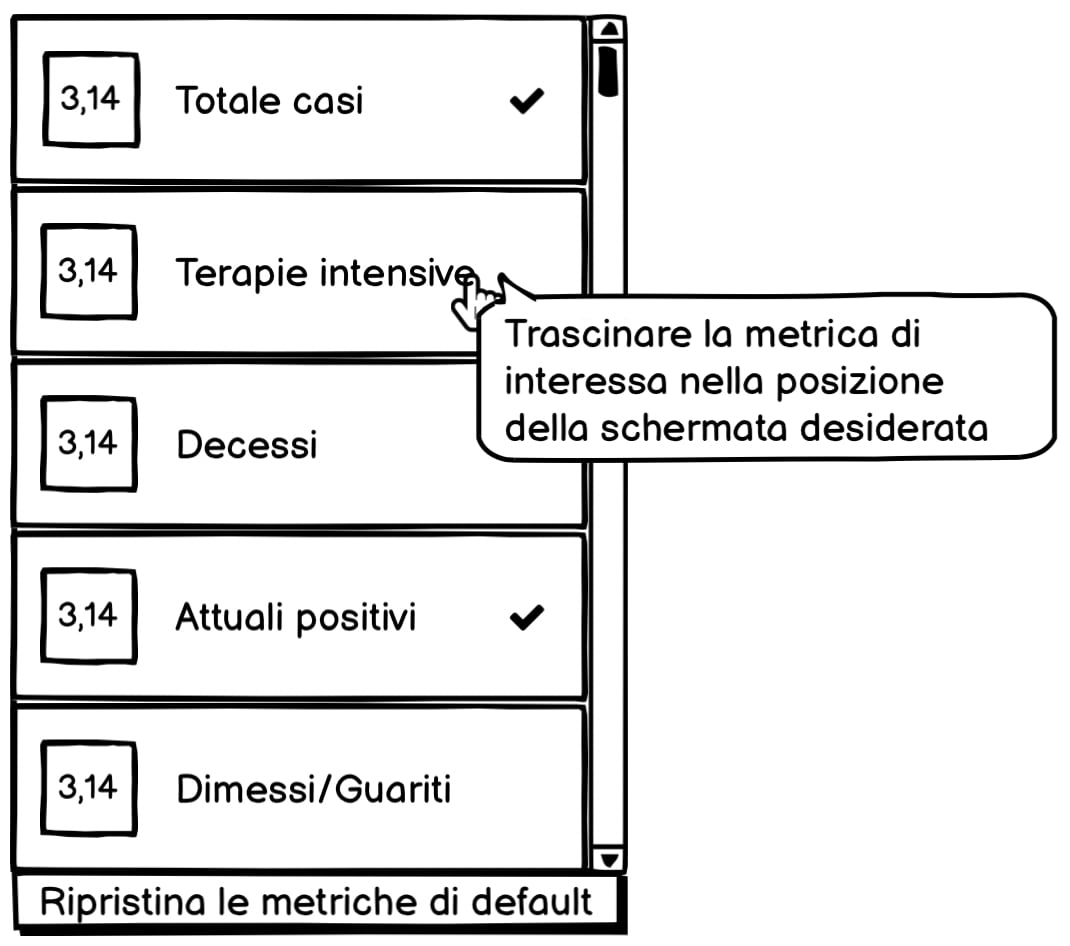
\includegraphics[width=0.5\textwidth]{wireframes/seleziona-metriche-tooltip}
        \caption{Tooltip in caso di click su un elemento della lista.}
        \label{fig:seleziona-metriche-tooltip}
    \end{subfigure}
    \caption{Seleziona metriche.}
\end{figure}


\paragraph{Seleziona data}
I widget per selezionare la data, apribili tramite il bottone tra le due frecce, sono di due tipi. Uno se la pagina richiede  di inserire un singolo giorno e l'altro se la pagina richiede di inserire  un range di date.\\

\begin{figure}[H]
    \begin{subfigure}[b]{0.5\textwidth}
        \centering
        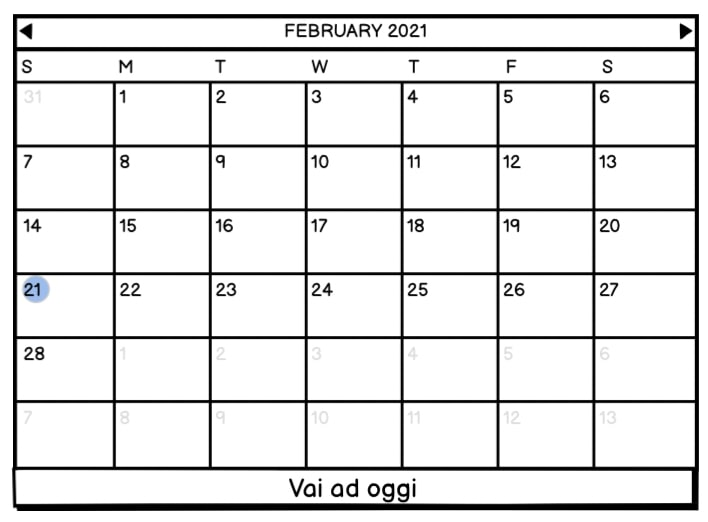
\includegraphics[width=0.5\textwidth]{wireframes/header-data-singola}
        \caption{Widget per selezionare una data singola.}
        \label{fig:header-data-singola}
    \end{subfigure}
\hfill
    \begin{subfigure}[b]{0.5\textwidth}
        \centering
        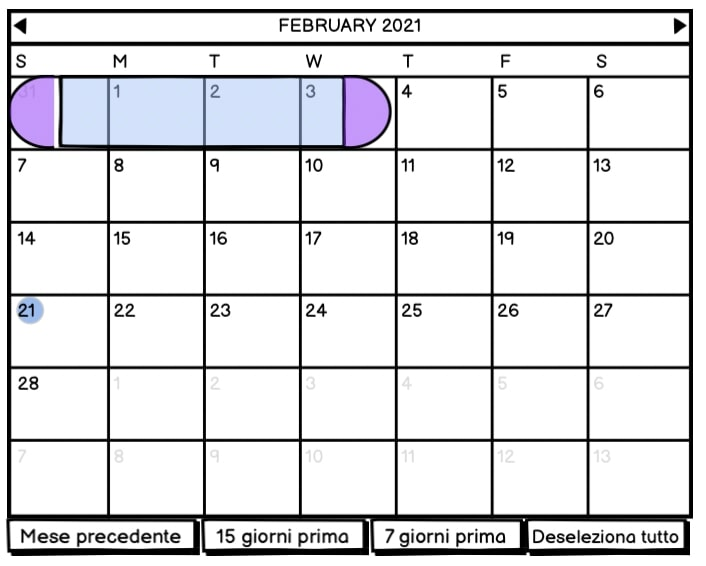
\includegraphics[width=0.5\textwidth]{wireframes/header-data-range}
        \caption{Widget per selezionare un range di date.}
        \label{fig:header-data-range}
    \end{subfigure}
    \caption{Widget per selzionare la data.}
\end{figure}

\begin{figure}[H]
    \centering
    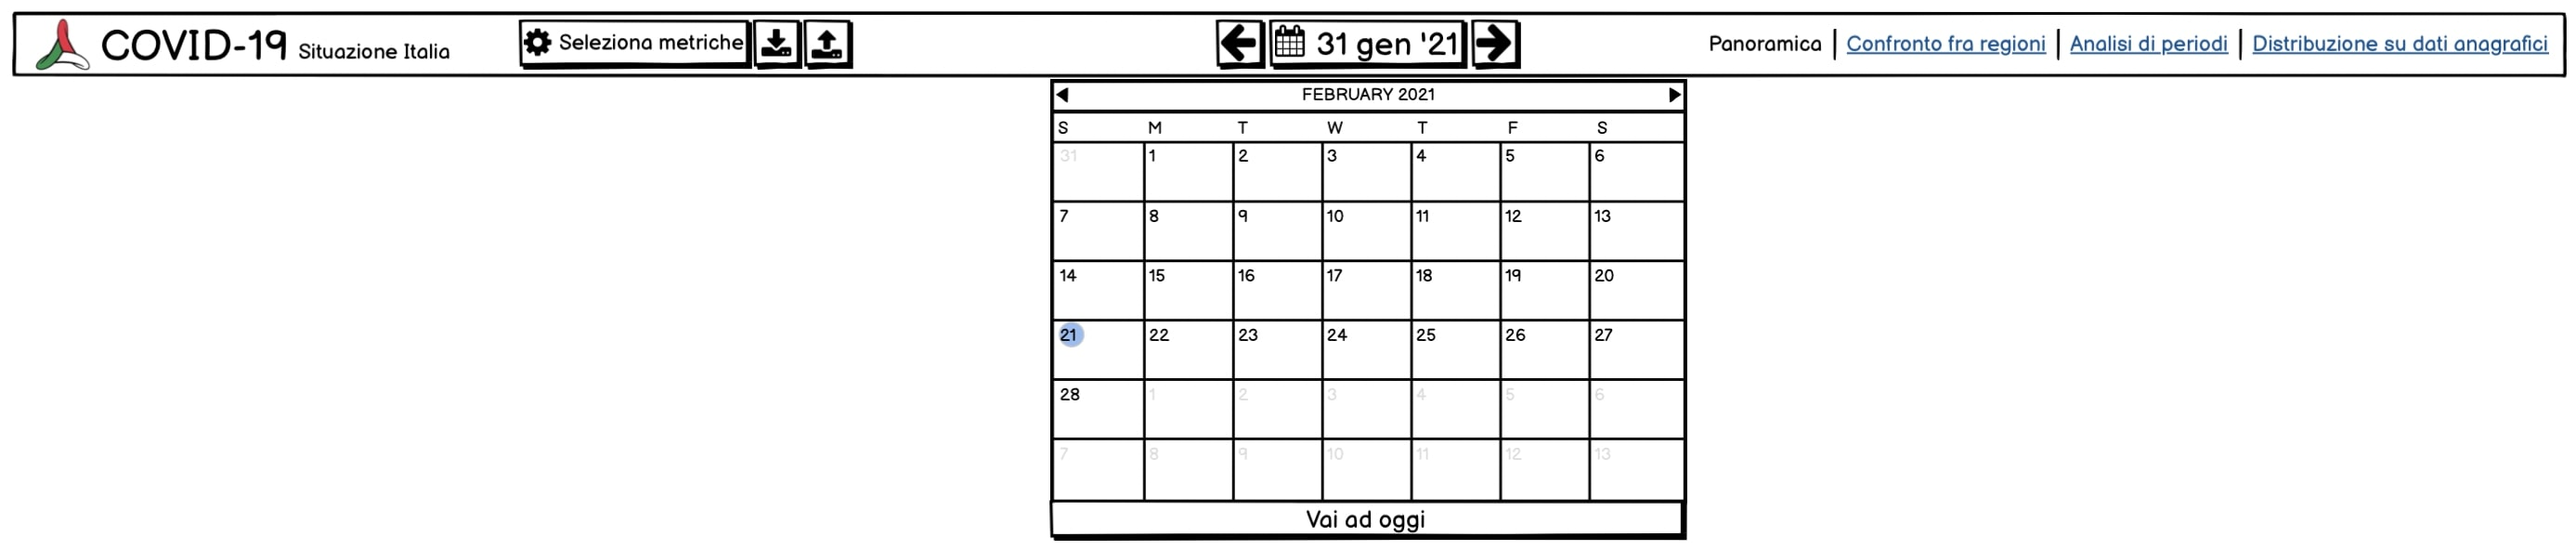
\includegraphics[width=1\columnwidth]{wireframes/header-data-aperta}
    \caption{Header con data aperta.}
    \label{fig:header-data-aperta}
\end{figure}

Nel widget per selezionare una data singola (\ref{fig:header-data-singola}) vi è un bottone per tornare rapidamente alla data odierna.\\
Nel widget per selezionare un range di date (\ref{fig:header-data-range}) vi sono diversi bottoni che permettono di velocizzare alcune operazioni come: andare al mese precednete, ai quindici giorni precedenti, ai sette giorni precedenti e per deselezionare il range.\\
In \ref{fig:header-data-aperta} vi è una dimostrazione di come il widget appare rispetto all'header.

\begin{figure}[H]
    \centering
    
\includegraphics[width=1\columnwidth]{wireframes/footer}
    \caption{Footer comune a tutte le schermate}
    \label{fig:footer}
\end{figure}

Nel footer (\ref{fig:footer}) vi sono alcune informarzioni e link per le pagine istituzionali e le fonti dai quali i dati sono stati recuperati; da destra ci sono:
\begin{itemize}
    \item logo della Repubblica Italiana;
    \item logo e nome della Protezione Civile;
    \item link alle fonti e data dell'ultimo aggiornamento;
    \item link ai siti istituzionali.
\end{itemize}

\subsubsection{Panoramica}\label{ss:panoramica}
\begin{figure}[H]
    \centering
    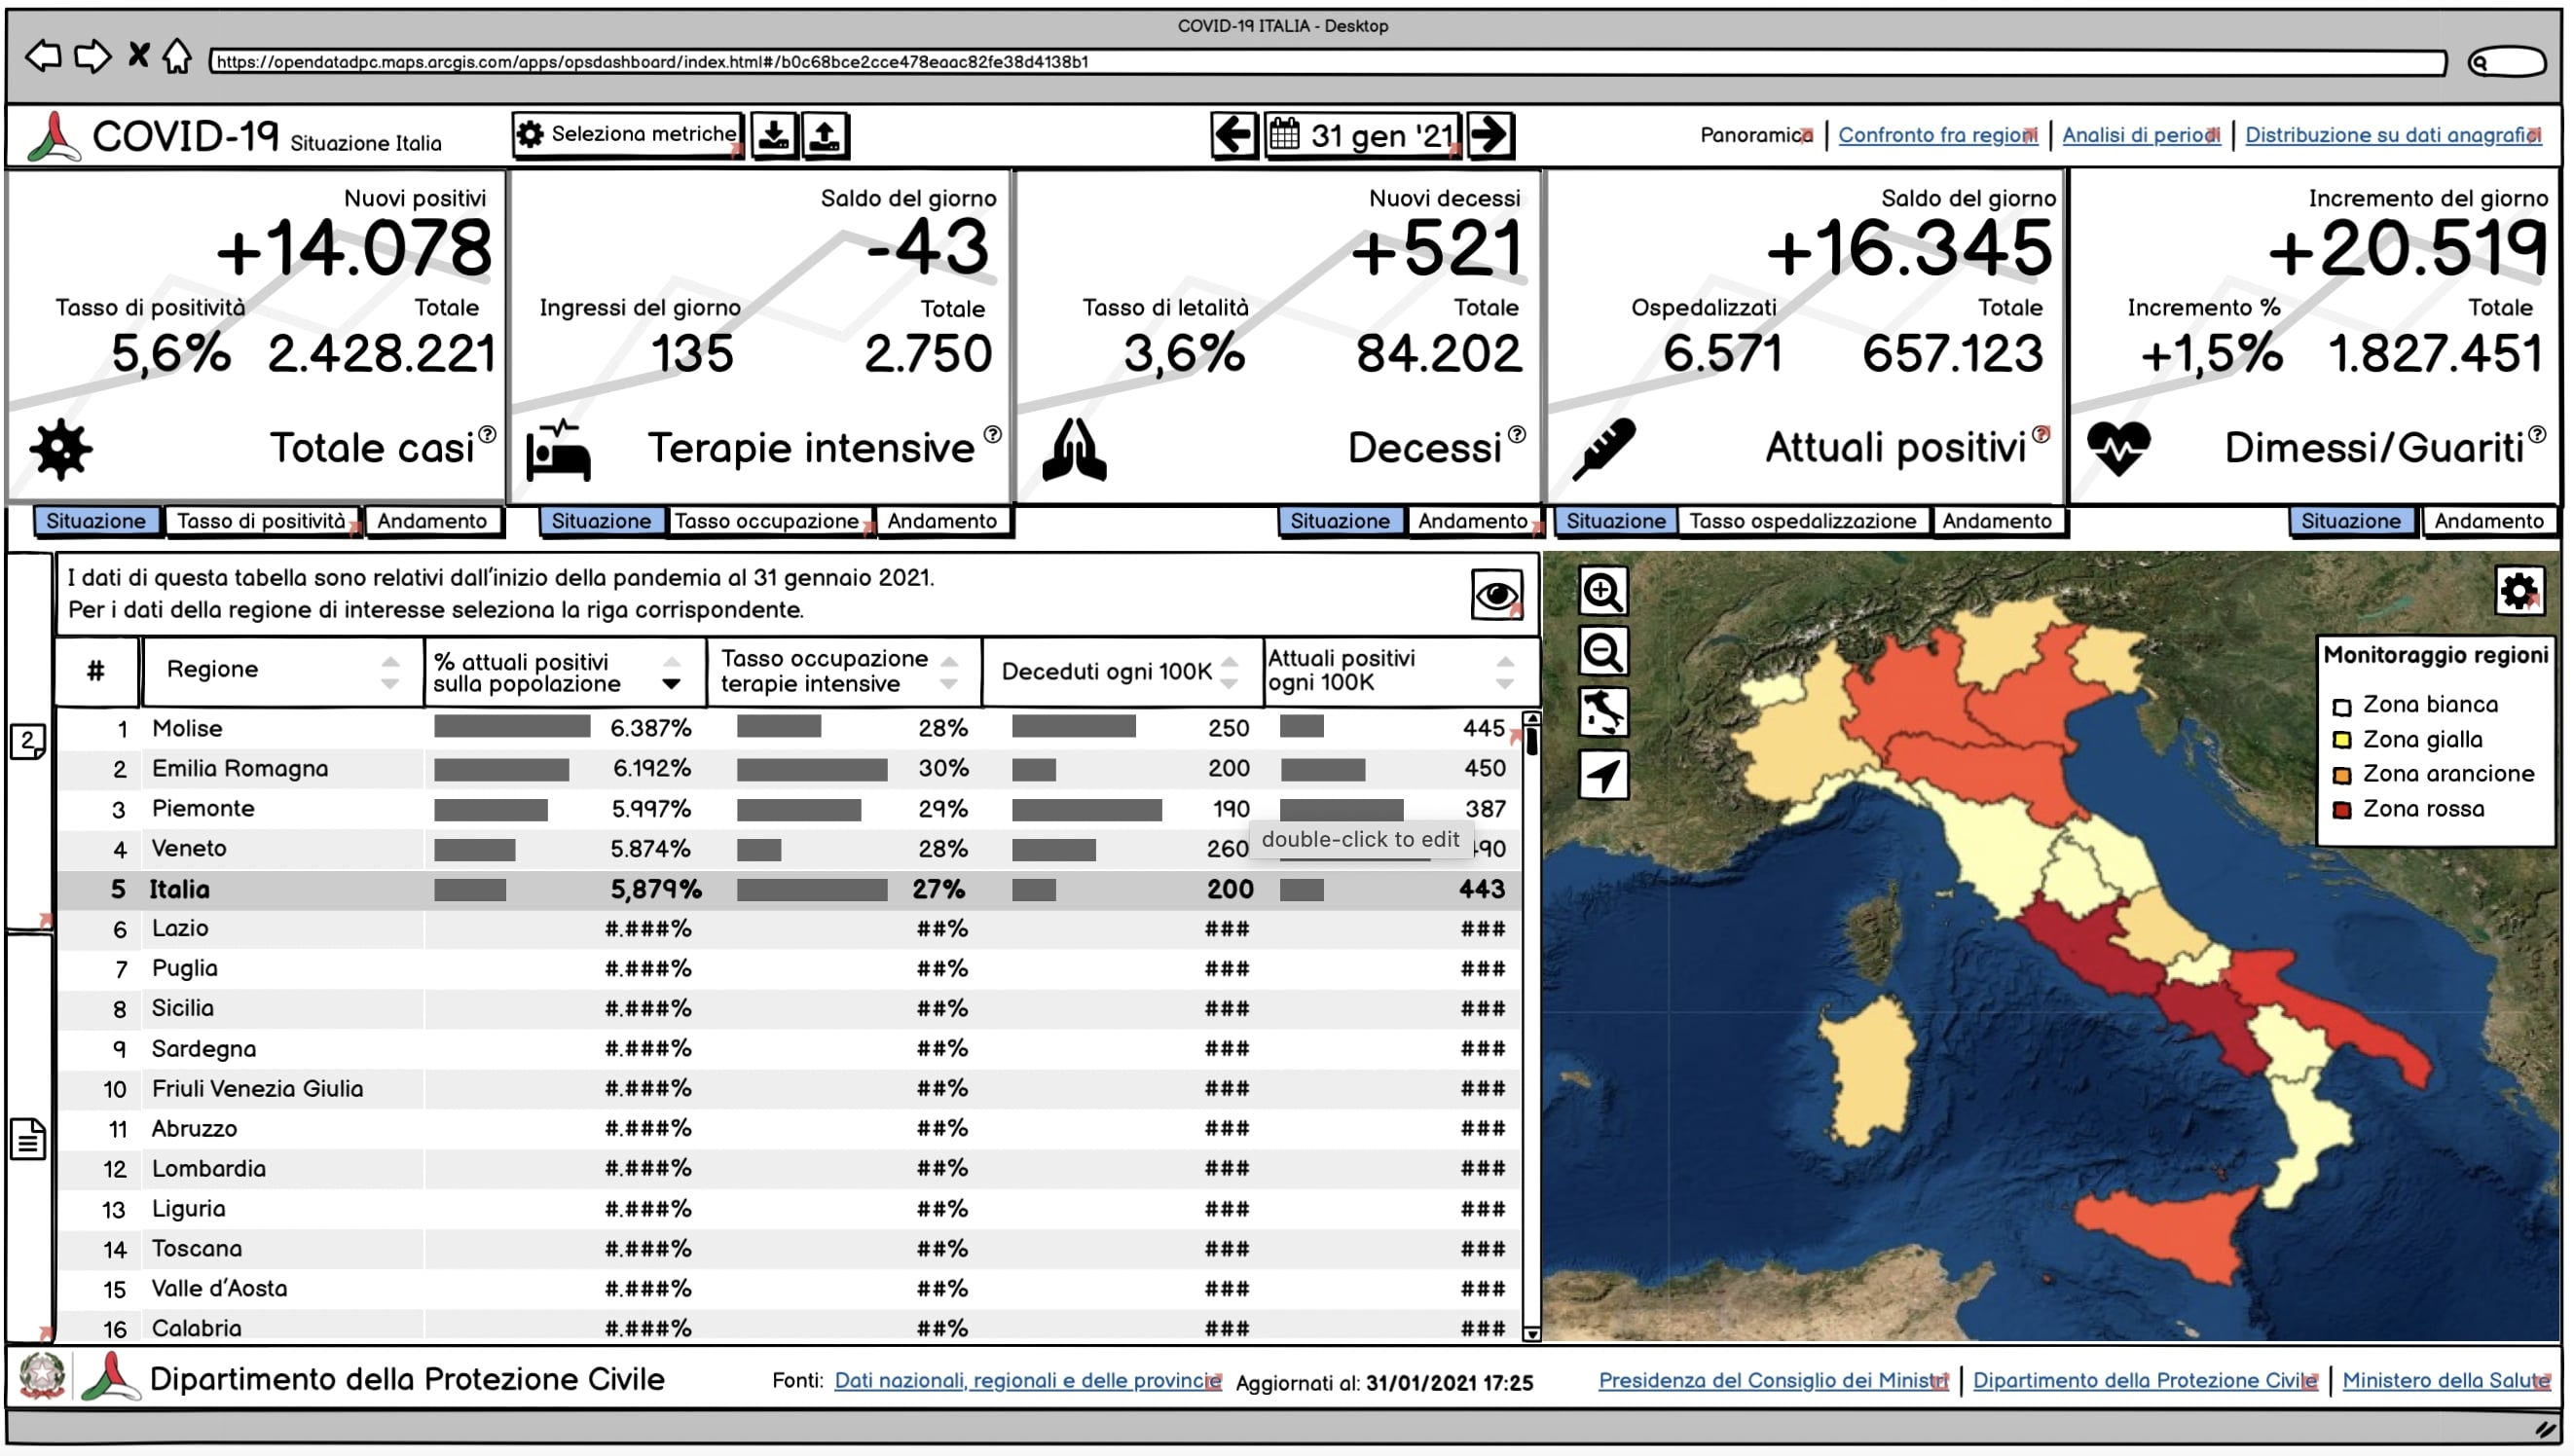
\includegraphics[width=1\columnwidth]{wireframes/panoramica}
    \caption{Schermata ``Panoramica''}
    \label{fig:panoramica}
\end{figure}
La schermata ``Panoramica'' è la prima schermata che un utente incontra aprendo la dashboard. \`E possibile dividere visivamente la schermata in due fasce: la fascia superiore che presenta cinque ``Box numerici'' e una fascia inferiore che presenta una tabella e una \textit{heat map}.\\

\paragraph{Box numerici}
\begin{figure}[H]
    \centering
    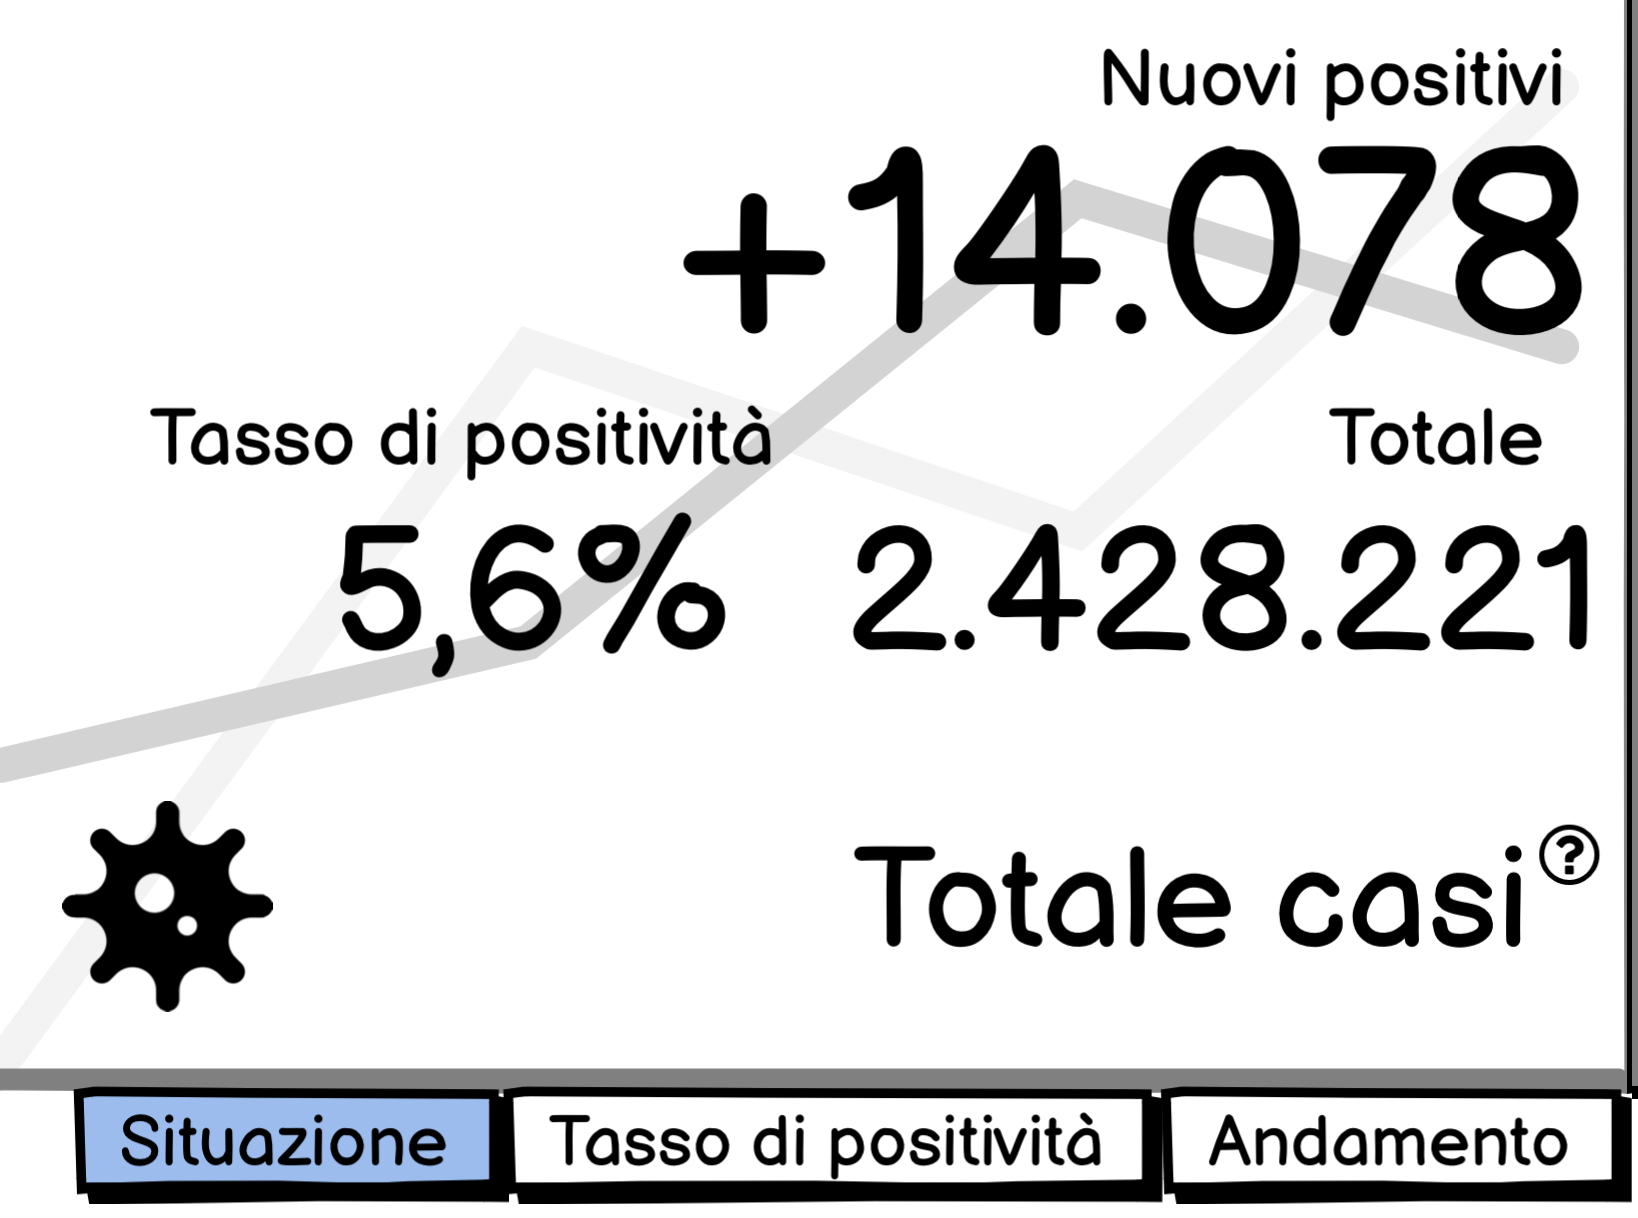
\includegraphics[width=0.5\columnwidth]{wireframes/box-numerico}
    \caption{Esempio di box numerico.}
    \label{fig:box-numerico}
\end{figure}

I cinque box numerici, di cui \ref{fig:box-numerico} ne è un esempio, sono composti dal nome della metrica in basso e con una dimensione del font maggiore rispetto alle altre etichette, due tre valori numerici, ognuno dei quali ha al di sopra un'etichetta per spiegare a cosa quel valore si riferisce. Vi è inoltre un'icona, utile per aiutare la memoria e diminuire il carico cognitivo in quanto semplifica il riconoscimento del box. Come sfondo del box vi è la curva che rappresenta l'andamento della metrica.\\
Al di sotto di ogni box numerico vi sono due o tre pulsanti che cambiano il contenuto del box numerico: il pulsante ``Andamento'' mostra un grafico con l'andamento della metrica (\ref{fig:box-andamento}), il pulsante ``Tasso di \dots'' mostra una \textit{gauge} (\ref{fig:box-gauge}) mentre il pulsante ``Situazione'' mostra il box numerico mostrato di default all'apertura della pagina.

\begin{figure}[H]
    \begin{subfigure}[b]{0.5\textwidth}
        \centering
        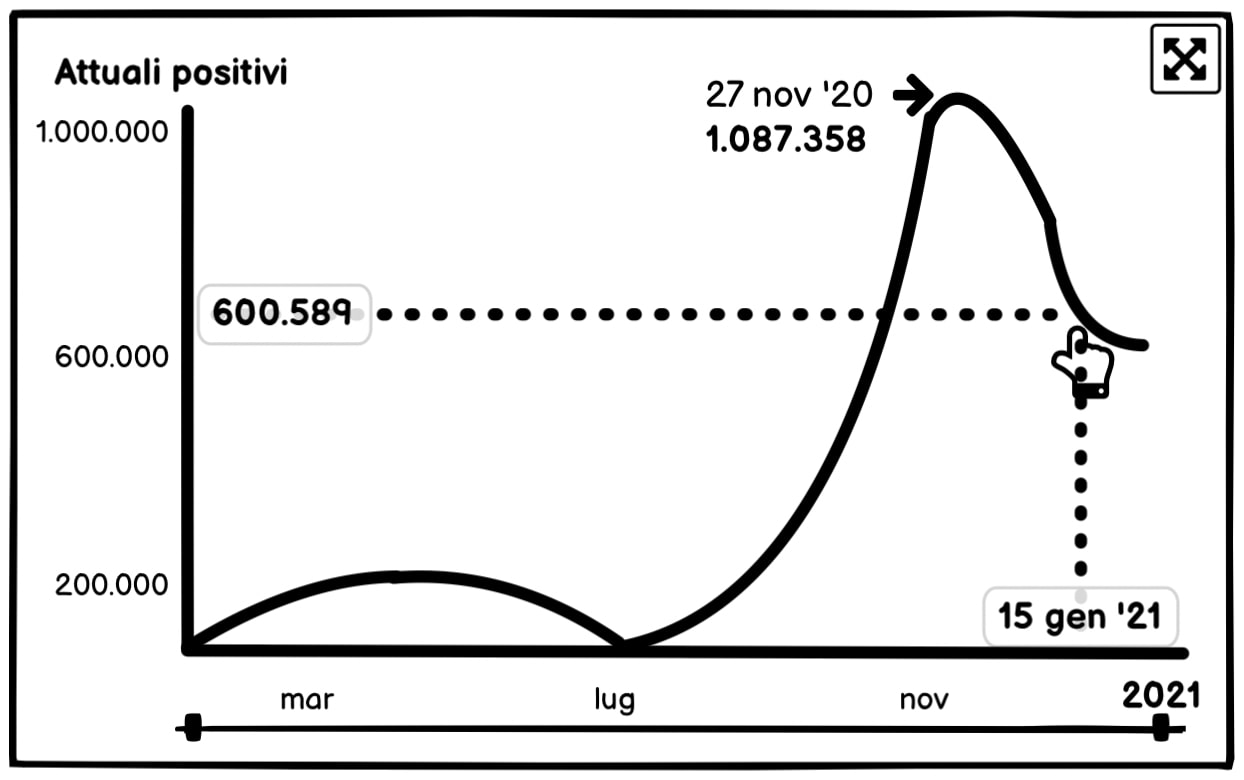
\includegraphics[width=1\textwidth]{wireframes/box-andamento}
        \caption{Box con grafico dell'andamento.}
        \label{fig:box-andamento}
    \end{subfigure}
\hfill
    \begin{subfigure}[b]{0.5\textwidth}
        \centering
        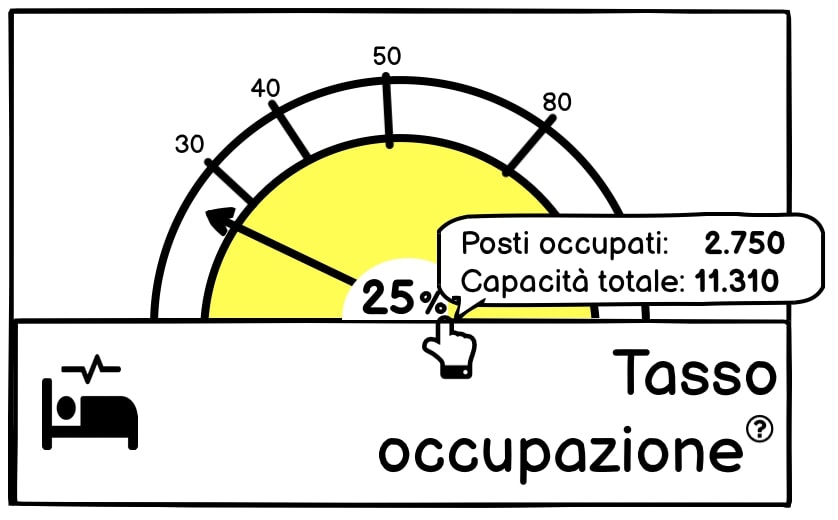
\includegraphics[width=1\textwidth]{wireframes/box-gauge}
        \caption{Box con gauge.}
        \label{fig:box-gauge}
    \end{subfigure}
    \caption{Viste alternative del ``Box numerico'' nella schermata ``Panoramica''.}
\end{figure}

\paragraph{Box con andamento}
I box con andamento possono avere due tipi di grafico in baso alla metrica rispetto alla quale si vuole osservare l'andamento: uno con una curva monotona crescente, utilizzato per mostrate l'andamento di metriche che possono solo salire (\ref{fig:box-andamento-monotono}) e un altro con una curva che non presenta monotonia (\ref{fig:box-andamento-no-monotonia}). 
\begin{figure}[H]
    \begin{subfigure}[b]{0.5\textwidth}
        \centering
        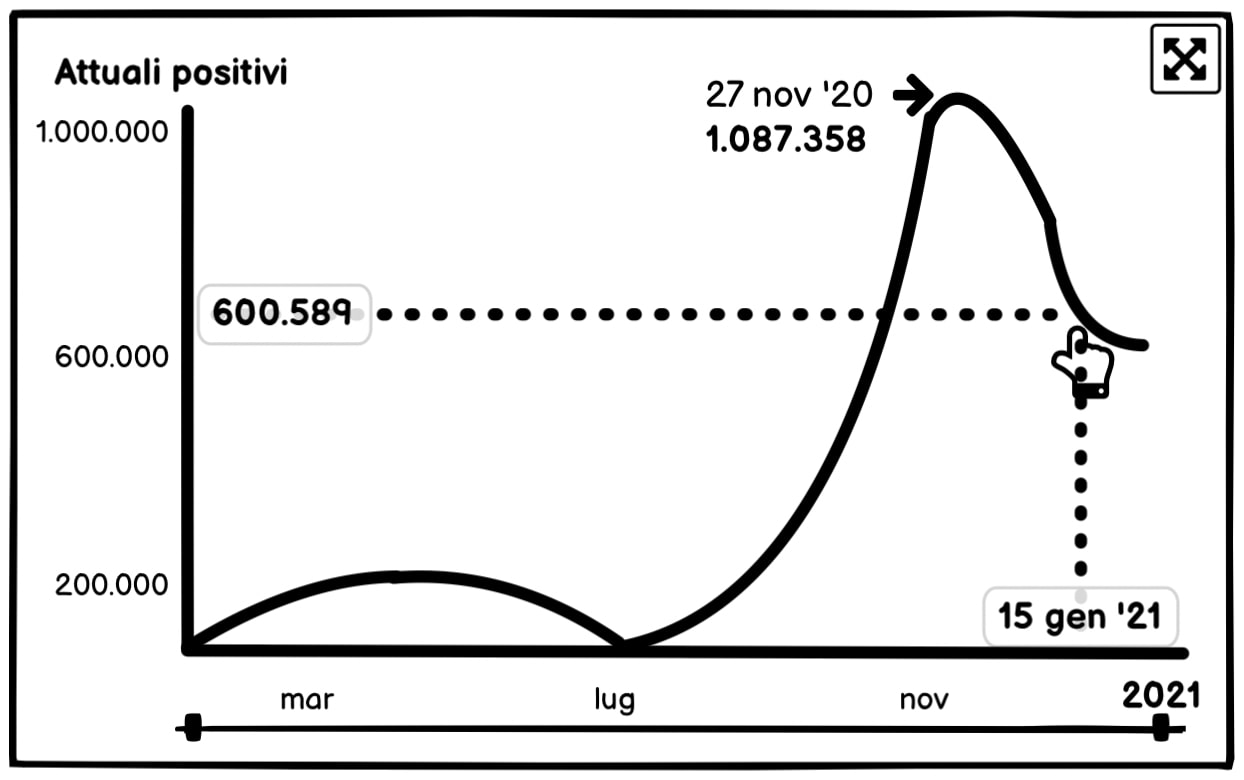
\includegraphics[width=1\textwidth]{wireframes/box-andamento}
        \caption{Box con grafico dell'andamento con una curva che non presenta monotonia.}
        \label{fig:box-andamento-no-monotonia}
    \end{subfigure}
\hfill
    \begin{subfigure}[b]{0.5\textwidth}
        \centering
        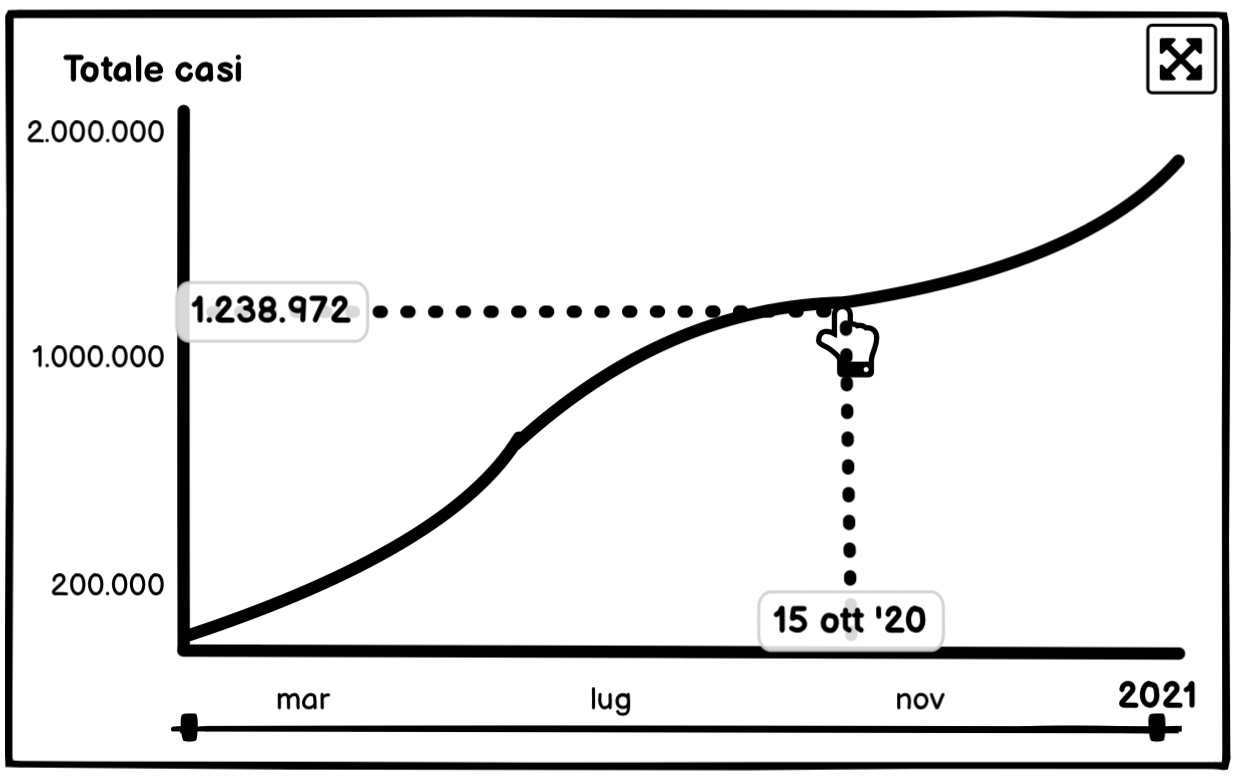
\includegraphics[width=1\textwidth]{wireframes/box-andamento-monotono}
        \caption{Box con grafico dell'andamento con una curva monotona crescente.}
        \label{fig:box-andamento-monotono}
    \end{subfigure}
    \caption{Differenti tipi di grafico dell'andamento di una metrica.}
\end{figure}

In \ref{fig:box-andamento-no-monotonia} è presente un'indicatore al valore massimo raggiunto, che, a differenza, in \ref{fig:box-andamento-monotono} non è presente.\\
Comune ad entrambi in grafici vi è uno slider vicino all'asse delle X con duplice selettore; questo slider può essere utilizzato per restringere il range di date che il grafico rappresente. Inoltre in caso si passi sopra al grafico con il cursore, compare un tooltip che indica con precisione i valori raggiunti il giorno indicato dalla proiezione sull'asse delle X.\\
In questi grafici è presente un pulsante in alto a destra che permette di visualizzare il grafico a pieno schermo, un esempio di come la schermata cambia lo si può vedere in \ref{fig:grafico-full-screen}. Lo stesso pulsante può essere utilizzato per far tornare il grafico alla sua dimensione originaria.
\begin{figure}[H]
    \centering
    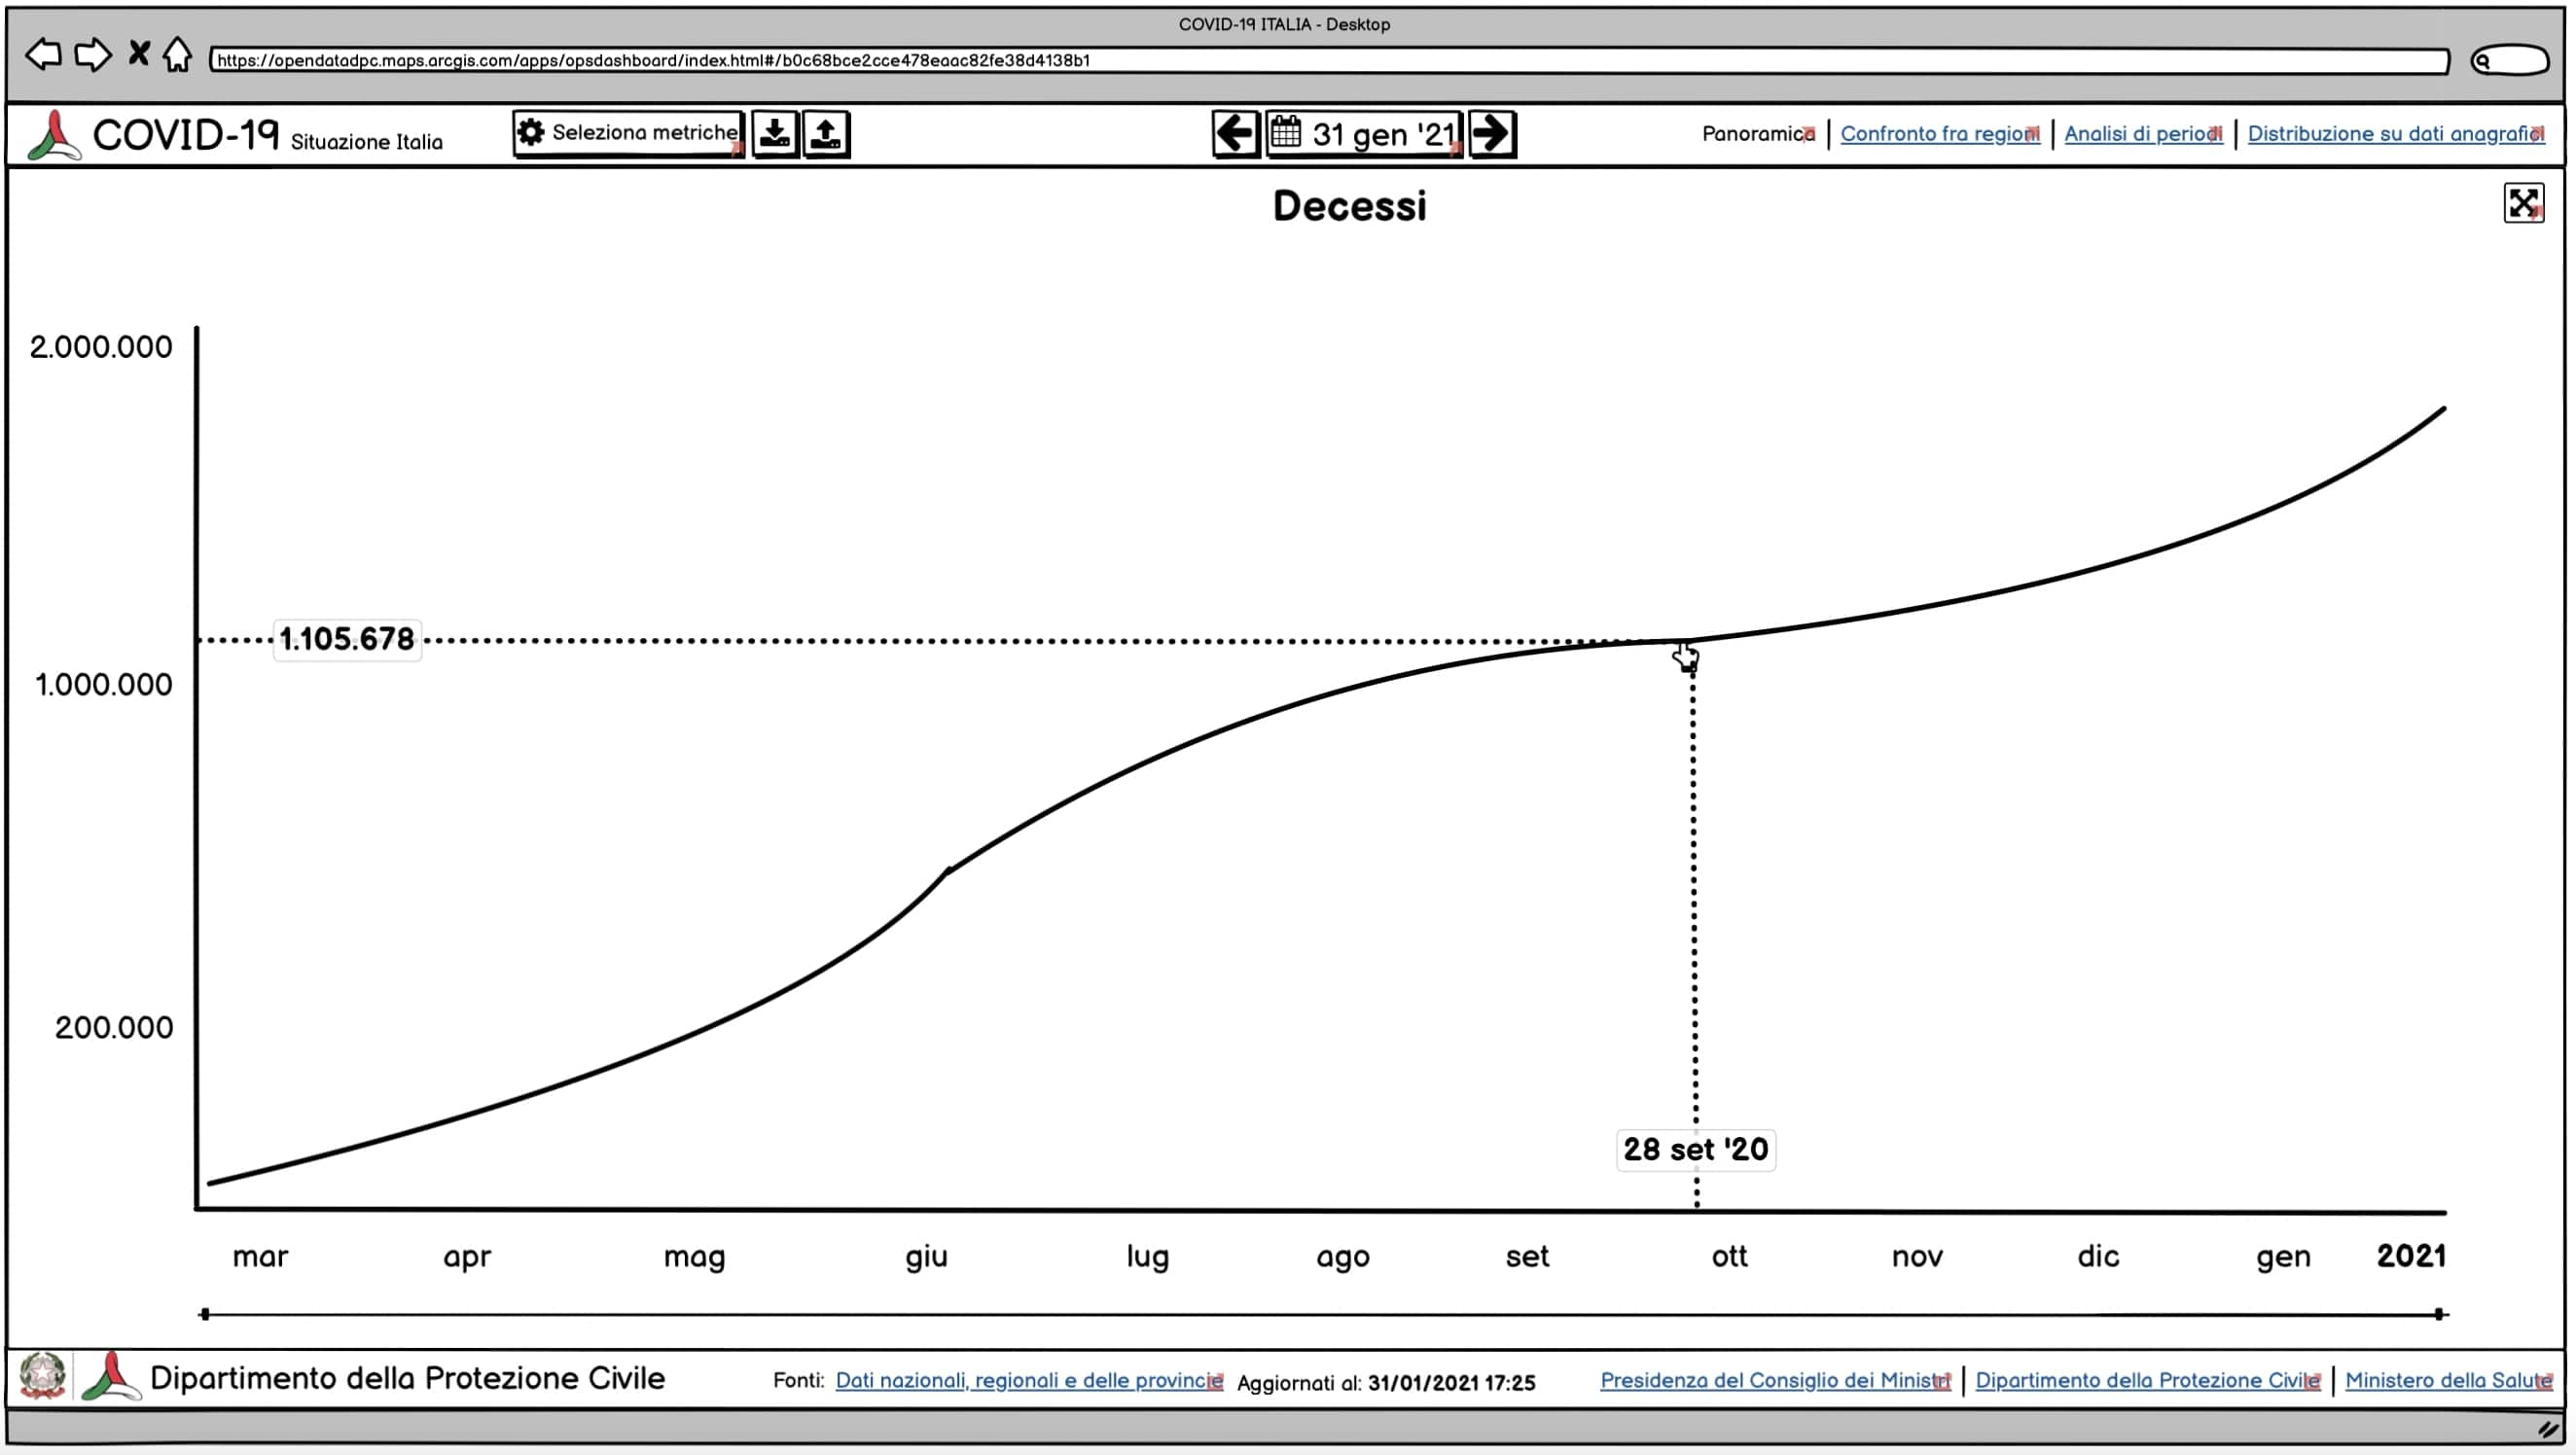
\includegraphics[width=0.7\columnwidth]{wireframes/grafico-full-screen}
    \caption{Grafico a pieno schermo}
    \label{fig:grafico-full-screen}
\end{figure}


\paragraph{Box con gauge}
I box con gauge sono utili per avere il colpo d'occhio di una specifica situazione (tasso di positività, tasso di occupazione delle terapie intensive, tasso di ospedalizzazioni). In caso si passi sopra alla gauge con il cursore, compare un tooltip che mostra i valori non percentuali di quella metrica.

\paragraph{Tabella}

\paragraph{Mappa}

\subsubsection{Confronto fra regioni}\label{ss:confronto-fra-regioni}

\subsubsection{Analisi di periodi}\label{ss:analisi-di-periodi}

\subsubsection{Distrubuzione su dati anagrafici}\label{ss:distribuzione-su-dati-anagrafici}
